% Provenance (never printed): see sources/outline_sources.md (Year 3:
% facies analysis, depositional models, Walther's law, well logs). Brief:
% sources/book5/BRIEFS.md, ch. 17. Curves from figdata/bachelor-3/well_logs.py
% (unit tops from figdata/shared/region.py). Exercise and problem values in
% the Book 5 scratch calculator calc/ch17.py. The well 瓦尔登-2, its logs and
% the channel architecture of its sandstone are invented.
\chapter{相模式}\label{ch:b3:facies-models}

取自一口深一千米井中的岩芯：一米厚的粗砂，
含交错层理，覆于截然的底面之上，向上变细为带有
根迹的粉砂，之上又是一层砂，覆于另一截然底面之上。地质学家读出一条河流
曾在其平原上蜿蜒流淌，而今那里已无河流。这一解读
依赖两种工具：一组\omterm{def:b3:facies-models:model}{相模式}，每一组概括同一环境的众多
现代及古代实例；以及一条定律，它把垂向的岩层序列
转化为相邻环境的分布图。

\begin{recall}
沉积相、沉积环境、床形、交错层理、
三类三角洲、浊流、浊积岩和递变层
均见于本科一年级分册中关于碎屑沉积及其
环境的章节；碳酸盐工厂、礁和碳酸盐台地见
其关于碳酸盐、硅质和蒸发岩沉积的章节；钻孔柱状图与
测井对比见其关于剖面的章节。孔隙度和
渗透率见中学课本。\omterm{def:b3:sequence-stratigraphy:parasequence}{准层序}、\omterm{def:b3:sequence-stratigraphy:parasequence}{海泛面}和
\omterm{def:b3:sequence-stratigraphy:tract}{体系域}见第~\ref{ch:b3:sequence-stratigraphy}~章。深水中的波浪
其运动随深度衰减，内容见物理学教材。
\end{recall}

\section{相、相序与沃尔瑟定律}\label{sec:b3:facies-models:walther}

沉积相依据岩芯或悬崖上可见的特征来描述：
粒度、分选、构造、化石和颜色。单一的相
很少具有判别性：交错层理砂可形成于河流、海滩、潮汐
水道和沙漠中。能够确定环境的，是一种相所伴生的
其他相，以及各相相互更替的顺序。

\begin{definition}[相组合与相序]\label{def:b3:facies-models:association}
称\emph{相组合}\index{相组合}为一组共同出现的相，
它们沉积于同一环境中，例如河道砂、
天然堤粉砂和带根的河漫滩泥。称\emph{相
序}\index{相序}为一个垂向的相序列，其中某种性质
逐渐向上变化；在\emph{向上变细
序列}\index{向上变细序列}中，粒度向上减小，
而在\emph{向上变粗序列}\index{向上变粗序列}中，
粒度向上增大。
\end{definition}

\begin{definition}[相模式]\label{def:b3:facies-models:model}
称\emph{相模式}\index{相模式}为对一种沉积环境的概括，
由众多现代及古代实例提炼而成，内容包括：
该环境所形成的相、它们的几何形态、侧向关系以及
所构成的\omterm{def:b3:facies-models:association}{相序}。它可作为与新实例进行比较的标准、
进一步观察的指南、新情境下的预测工具，以及
解释沉积环境的依据。
\end{definition}

连接侧向与垂向的桥梁是一条定律。相邻的
环境在任一时刻并排分布：海滩紧邻\omterm{def:b3:facies-models:shoreface}{临滨}，
\omterm{def:b3:facies-models:shoreface}{临滨}紧邻外陆架泥。当岸线移动时，
每一环境都会覆盖在其相邻环境之上。

\begin{theorem}[沃尔瑟定律]\label{thm:b3:facies-models:walther}
在整合的层序中，若沉积无明显间断，且没有
侵蚀面，则上下直接相接的相
沉积于当时并排分布的环境中。
\end{theorem}

\begin{proof}
考虑若干环境带，每一环境带都是平行于岸线的条带，它们
在盆地中共同迁移，同时盆底沉降或海平面上升。
在某一固定地点，各环境带依次经过，顺序
与其并排时的顺序一致，每一环境带都在其前一环境带的
沉积之上留下自己的沉积。若沉积连续，则
沉积的垂向顺序即为环境带的侧向顺序。
间断或侵蚀面会打断这一论证：在间隔期间经过的环境带
未留下任何沉积，或其沉积已被移除，于是
来自非相邻环境的相彼此接触。
\end{proof}

\begin{omfigure}
\begin{tikzpicture}[font=\scriptsize, x=1cm, y=1cm]
% environments side by side, with a shoreline that moves seaward
\fill[yellow!35!brown!25] (0,0) rectangle (3,0.5);
\fill[yellow!30] (3,0) rectangle (4.4,0.5);
\fill[yellow!50!orange!30] (4.4,0) rectangle (6.4,0.5);
\fill[black!20] (6.4,0) rectangle (9,0.5);
\draw (0,0) rectangle (9,0.5);
\foreach \x in {3,4.4,6.4} {\draw (\x,0) -- (\x,0.5);}
\node at (1.5,0.25) {海岸平原};
\node at (3.7,0.25) {海滩};
\node at (5.4,0.25) {临滨};
\node at (7.7,0.25) {外陆架泥};
\draw[->, thick] (3.2,0.9) -- (5.2,0.9) node[right] {环境带向海迁移};
\node[anchor=south] at (4.5,1.2) {(a) 并排分布的环境};
% vertical succession at a place
\begin{scope}[xshift=11cm, yshift=-1.2cm]
\fill[black!20] (0,0) rectangle (0.9,0.8);
\fill[yellow!50!orange!30] (0,0.8) -- (0.9,0.8) -- (1.3,1.8) -- (0,1.8) -- cycle;
\fill[yellow!30] (0,1.8) rectangle (1.4,2.4);
\fill[yellow!35!brown!25] (0,2.4) rectangle (1.0,3.1);
\draw (0,0) -- (0.9,0) -- (0.9,0.8) -- (1.3,1.8) -- (1.4,1.8) -- (1.4,2.4) -- (1.0,2.4) -- (1.0,3.1) -- (0,3.1) -- cycle;
\node[anchor=west] at (1.6,0.4) {外陆架泥};
\node[anchor=west] at (1.6,1.3) {临滨砂};
\node[anchor=west] at (1.6,2.1) {海滩};
\node[anchor=west] at (1.6,2.75) {海岸平原};
\draw[->] (-0.3,0) -- (-0.3,3.1) node[above] {向上};
\node[anchor=north, align=center] at (0.9,-0.1) {(b) 某一地点的 \\相序};
\end{scope}
\end{tikzpicture}

\par\smallskip{\small 瓦尔特定律。（a）环境沿
剖面并列分布；（b）随各相带向海推移，某一地点先接受离岸泥，
再接受\omterm{def:b3:facies-models:shoreface}{临滨}砂、海滩砂和海岸平原沉积，即
按相带次序向上变粗的序列（柱状图中宽度表示
颗粒更粗）。}\label{fig:b3:facies-models:walther}
\end{omfigure}

该定律可双向应用。海退时，各相带按向海次序
向上叠置，海侵时则按相反次序叠置；由岩芯中读取的垂向序列
可给出当时邻近环境的平面分布。该定律
恰在第~\ref{ch:b3:sequence-stratigraphy}~章标示的关键界面处失效：
在\omterm{def:b3:sequence-stratigraphy:sequence}{层序界面}处，暴露与侵蚀使河流砂覆于
陆架泥之上；在\omterm{def:b3:sequence-stratigraphy:parasequence}{海泛面}处，离岸泥直接覆于
海岸平原之上。

\section{河流}\label{sec:b3:facies-models:rivers}

\begin{definition}[辫状河与曲流河]\label{def:b3:facies-models:rivers}
\emph{辫状河}\index{辫状河}在若干浅窄的河道中流动，
河道绕沙坝分叉又汇合，发育于坡度较陡的平原上，载荷中粗颗粒丰富，
流量变化大。\emph{曲流河}\index{曲流河}在单一的蜿蜒河道中流动，
发育于坡度较缓的平原上，携带的细粒沉积物较多；
它通过侵蚀每个弯道的凹岸并在凸岸沉积而迁移。
凸岸处的沉积体称为
\emph{点沙坝}\index{点沙坝}。\emph{河道改道}\index{河道改道}指河道弃用原有
河道、穿过河漫滩另辟新道，通常发生在洪水
冲破天然堤之后。
\end{definition}

\omterm{def:b3:facies-models:rivers}{点沙坝}随弯道迁移而向侧向增长，因此在任一地点，它都记录了
河道自下而上的横截面：底部为侵蚀底面上的最粗粒碎屑滞留层，
其上为深槽沙丘形成的交错层理砂，
再向上为沙坝浅部形成的带波痕细砂，
最后是带根系与土壤的河漫滩粉砂和泥。依据瓦尔特定律，这一
\omterm{def:b3:facies-models:association}{向上变细序列}厚仅数米，其厚度与
河道深度相当。\omterm{def:b3:facies-models:rivers}{辫状河}则留下叠置的交错层理砂与
砾石席状体，泥质很少，粒度自下而上几乎不变，其细粒组分
已被搬运走。\omterm{def:b3:facies-models:rivers}{河道改道}使河道带在平原上迁移，
因此河道砂体随机地叠置于河漫滩泥之间，
并以陡直的侵蚀底面为界。

\begin{omfigure}
\begin{tikzpicture}[font=\scriptsize, x=1cm, y=1cm]
% (a) braided plan
\begin{scope}
\fill[yellow!35!brown!20] (0,0) rectangle (4.6,2.4);
\draw[omDef!60, line width=1.6pt] (0,1.2) .. controls (0.8,1.6) and (1.4,0.6) .. (2.3,1.0) .. controls (3.0,1.3) and (3.6,0.7) .. (4.6,1.0);
\draw[omDef!60, line width=1.6pt] (0,1.2) .. controls (0.8,0.8) and (1.6,1.9) .. (2.4,1.6) .. controls (3.2,1.3) and (3.8,1.9) .. (4.6,1.6);
\draw[omDef!60, line width=1.2pt] (1.2,1.25) .. controls (1.8,1.5) and (2.6,1.2) .. (3.3,1.35);
\fill[yellow!45] (1.5,1.15) ellipse (0.35 and 0.12);
\fill[yellow!45] (3.0,1.25) ellipse (0.4 and 0.12);
\node[anchor=south] at (2.3,2.45) {(a) 辫状河};
\end{scope}
% (b) meandering plan
\begin{scope}[xshift=5.4cm]
\fill[green!30!black!12] (0,0) rectangle (4.6,2.4);
\draw[omDef!60, line width=2pt] (0,1.2) .. controls (0.6,2.2) and (1.4,2.2) .. (1.6,1.2) .. controls (1.8,0.2) and (2.8,0.2) .. (3.0,1.2) .. controls (3.2,2.2) and (4.0,2.2) .. (4.6,1.2);
\fill[yellow!45] (0.8,1.45) ellipse (0.3 and 0.2);
\fill[yellow!45] (2.3,0.95) ellipse (0.3 and 0.2);
\fill[yellow!45] (3.8,1.45) ellipse (0.3 and 0.2);
\node at (2.3,0.95) {pb};
\draw[omDef!40, line width=1pt, densely dashed] (0.4,0.2) .. controls (1.0,0.7) and (1.6,0.4) .. (2.0,0.1);
\node[anchor=west, font=\tiny] at (2.6,2.15) {河漫滩};
\node[anchor=south] at (2.3,2.45) {(b) 曲流河};
\end{scope}
% logs
\begin{scope}[xshift=10.8cm]
\fill[yellow!45] (0,0) -- (1.2,0) -- (1.2,2.0) -- (0,2.0) -- cycle;
\draw (0,0) -- (1.2,0) -- (1.15,0.6) -- (1.2,0.65) -- (1.1,1.3) -- (1.2,1.35) -- (1.15,2.0) -- (0,2.0) -- cycle;
\node[anchor=north] at (0.6,-0.05) {辫状河};
\end{scope}
\begin{scope}[xshift=12.6cm]
\fill[yellow!45] (0,0) -- (1.2,0) -- (1.1,0.9) -- (0.45,1.6) -- (0,1.6) -- cycle;
\fill[green!30!black!15] (0,1.6) rectangle (0.3,2.2);
\draw (0,0) -- (1.2,0) -- (1.1,0.9) -- (0.45,1.6) -- (0.3,1.6) -- (0.3,2.2) -- (0,2.2) -- cycle;
\draw[decorate, decoration={snake, amplitude=0.4mm, segment length=1.5mm}] (0,0) -- (1.2,0);
\node[anchor=north] at (0.6,-0.05) {点沙坝};
\node[anchor=west, font=\tiny] at (0.35,1.9) {根系};
\end{scope}
\end{tikzpicture}

\par\smallskip{\small （a）\omterm{def:b3:facies-models:rivers}{辫状河}：若干河道环绕由
砂和砾石组成的沙坝。（b）\omterm{def:b3:facies-models:rivers}{曲流河}：单一蜿蜒河道，\omterm{def:b3:facies-models:rivers}{点沙坝}（pb）
位于凸岸，虚线为\omterm{def:b3:facies-models:rivers}{河道改道}遗留的废弃河道。右侧为
沉积物粒度柱状图（宽度表示颗粒更粗）：叠置的砂席状体，
粒度自下而上变化很小（\omterm{def:b3:facies-models:rivers}{辫状河}）；\omterm{def:b3:facies-models:rivers}{曲流河}的\omterm{def:b3:facies-models:rivers}{点沙坝}则为底面陡直、
向上变细的序列，顶部覆有带根系的
河漫滩泥。}\label{fig:b3:facies-models:rivers}
\end{omfigure}

\section{岸线、三角洲与陆架}\label{sec:b3:facies-models:shelves}

本科一年级分册中的三角洲，无论受河流、波浪或潮汐控制，
都以相同机制向外推进：河口在水流减缓处沉积其载荷，
三角洲前缘向海进积，覆于自身的前三角洲泥之上。
进积的三角洲前缘或\omterm{def:b3:facies-models:shoreface}{临滨}面，依据瓦尔特定律，将形成
向上变粗的序列：离岸泥、泥与风暴砂互层、
\omterm{def:b3:facies-models:shoreface}{临滨}砂、海滩。上一章中的每个\omterm{def:b3:sequence-stratigraphy:parasequence}{准层序}都是这样的一个
序列。

\begin{definition}[临滨与波浪基面]\label{def:b3:facies-models:shoreface}
\emph{临滨}\index{临滨}是位于海滩向海一侧的斜坡地带，
波浪在此持续改造海底。其底界为
\emph{正常浪基面}\index{正常浪基面}，即正常波浪
不再搅动底部沉积物的深度。
\emph{风暴浪基面}\index{风暴浪基面}是风暴波浪所能到达的更深界限；
两者之间，泥在平静天气下沉降，
风暴期间则被改造为砂层。风暴浪基面以下，海底不受波浪扰动。
\end{definition}

\begin{omfigure}
\begin{tikzpicture}[font=\scriptsize, x=1cm, y=1.6cm]
\fill[omSea!60] (0,2.2) -- (13,2.2) -- (13,0.2) -- (5.5,0.9) -- (2.0,1.9) -- (0.6,2.2) -- cycle;
\fill[yellow!40] (0,2.4) -- (0.6,2.2) -- (2.0,1.9) -- (5.5,0.9) -- (5.5,0.0) -- (0,0.0) -- cycle;
\fill[black!18] (5.5,0.9) -- (13,0.2) -- (13,0) -- (5.5,0) -- cycle;
\draw[thick] (0,2.4) -- (0.6,2.2) -- (2.0,1.9) -- (5.5,0.9) -- (13,0.2);
\draw[omDef] (0,2.2) -- (13,2.2);
\draw[omDef, densely dashed] (1.6,1.97) -- (13,1.97);
\draw[omDef, densely dashed] (5.5,0.9) -- (13,0.9);
\node[omDef, anchor=north west] at (9.3,1.95) {正常浪基面};
\node[omDef, anchor=north west] at (9.3,0.88) {风暴浪基面};
\node[anchor=south] at (0.5,2.42) {海滩};
\node at (1.8,1.35) {临滨};
\node at (4.3,0.45) {离岸过渡带};
\node at (9.0,0.15) {离岸泥};
\node[align=center] at (7.4,1.45) {风暴砂层，\\ 丘状交错层理};
\end{tikzpicture}

\par\smallskip{\small 波浪主导海岸剖面示意图（垂向比例大幅夸大）。
\omterm{def:b3:facies-models:shoreface}{正常浪基面}以上，\omterm{def:b3:facies-models:shoreface}{临滨}砂层每天都被改造；
两个浪基面之间，泥与风暴沉积的砂层交替出现；
\omterm{def:b3:facies-models:shoreface}{风暴浪基面}以下，泥
逐渐沉积。}\label{fig:b3:facies-models:shoreface}
\end{omfigure}

深水中，波浪的轨道运动按 $e^{-2\pi z/\lambda}$ 随深度 $z$ 衰减，
其中 $\lambda$ 为波长：在半个波长深处，
它仍保留表面振幅的 \qty{4}{\percent}，这决定了浪基面的
尺度。取自加勒比海、墨西哥湾和西大西洋的
二百多万条浮标波谱记录显示，避风海域的众数波长约为
\qty{75}{m}，开阔陆缘约为 \qty{110}{m}。
并表明，对数周至数年取平均后，波长并不会分裂为
“正常天气”与“风暴”两类：波浪搅动海底的概率
随水深变浅而稳步上升。两个浪基面仍是描述剖面分带的
有用术语，但它们并非截然分明的深度。
% ledger: losspeters10:wavebase

\begin{definition}[丘状交错层理]\label{def:b3:facies-models:hcs}
\emph{丘状交错层理}\index{丘状交错层理}是
一种细砂层的层理，由平缓弯曲的纹层构成，既有上凹的
（洼地）也有上凸的（丘），纹层以低角度相互切割，
并在侧向上增厚或变薄，波长为一米至数米。它
由风暴波浪的振荡流与复合流形成，位于
\omterm{def:b3:facies-models:shoreface}{正常浪基面}与\omterm{def:b3:facies-models:shoreface}{风暴浪基面}之间。
\end{definition}

\begin{inthefield}[志留纪陆架上的风暴层]
\begin{minipage}[t]{0.42\linewidth}\vspace{0pt}
在新斯科舍省的阿里赛格组中，细砂岩层夹在
较暗的泥岩之间。研究此类层的地质学家能辨认出低缓、弯曲、
相互切割的\omterm{def:b3:facies-models:hcs}{丘状交错层理}纹层：每一层记录了
一次搅动陆架的风暴，该处位于日常波浪所不及之处，而其间的泥
则记录了风暴之间漫长的平静期。
\end{minipage}\hfill
\begin{minipage}[t]{0.54\linewidth}\vspace{0pt}
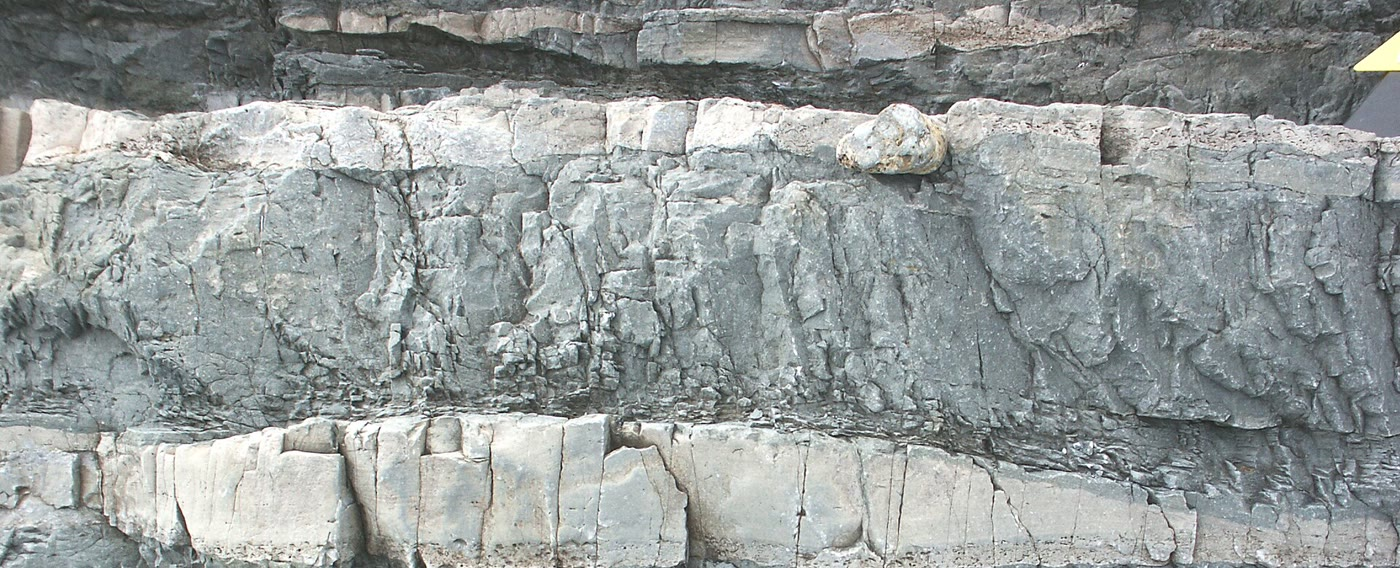
\includegraphics[width=\linewidth]{images/book5/b3-hummocky-cross-stratification.jpg}

{\scriptsize 新斯科舍省阿里赛格组（志留纪）中的\omterm{def:b3:facies-models:hcs}{丘状交错层理}，
位于阿里赛格附近。照片：Michael C. Rygel，CC BY-SA 3.0
（裁剪）。}
\end{minipage}
\end{inthefield}
% ledger: photo:b3-hcs

潮汐占主导时，相随之改变：涨潮与落潮流形成
方向相反的交错层，每次平潮时都有泥质披覆层沉降，
披覆层之间层束的厚度随
大小潮周期而增减。潮汐河道、潮坪与砂脊
各有自己的模式，建立方式相同。

\section{深水}\label{sec:b3:facies-models:deep}

减速的浊流按沉降顺序沉积其载荷：
最粗的颗粒先沉，最细的颗粒最后沉。一个完整的浊积岩层
以五个分段呈现这一顺序。

\begin{definition}[鲍马序列]\label{def:b3:facies-models:bouma}
\emph{鲍马序列}\index{鲍马序列}是浊积岩层中理想的
分段序列，自下而上为：Ta，块状或递变砂，位于
侵蚀底面之上，带有槽模与工具痕；Tb，平行纹层砂；Tc，
波纹交错层理与卷曲纹层细砂；Td，平行纹层粉砂；
Te，泥，部分来自浊流，部分来自
两股水流之间的缓慢沉降。
\end{definition}

很少有岩层能显示全部五个分段：靠近物源时水流快，留下较厚的
Ta 分段，其上部被下一股水流侵蚀；远离物源时，只剩
较细的 Tc 至 Te 分段。因此，该序列记录了
一股水流的减弱，而岩层沿扇体的变化记录了
水流随距离的减弱。

\begin{definition}[海底扇]\label{def:b3:facies-models:fan}
\emph{海底扇}\index{海底扇}是一种沉积锥体，位于
大陆坡坡脚，由海底峡谷供给：上扇为一条主河道，
位于天然堤之间；中扇为终止于砂叶的分支河道，
下扇为薄层浊积岩，逐渐过渡为盆底泥。
\end{definition}

沿陆缘，由海洋环流驱动的深层水流
将斜坡上的细粒沉积改造为等深流积岩、丘与漂丘，
它们由生物扰动的粉砂与泥构成，沿等深线而非
沿坡向下生长。

\begin{omfigure}
\begin{tikzpicture}[font=\scriptsize, x=1cm, y=1cm]
% (a) Bouma log
\begin{scope}
\fill[yellow!45] (0,0) -- (1.6,0) -- (1.6,1.2) -- (0,1.2) -- cycle;
\fill[yellow!35] (0,1.2) rectangle (1.3,1.8);
\fill[yellow!25] (0,1.8) rectangle (1.0,2.4);
\fill[black!12] (0,2.4) rectangle (0.7,2.8);
\fill[black!25] (0,2.8) rectangle (0.4,3.3);
\draw (0,0) -- (1.6,0) -- (1.6,1.2) -- (1.3,1.2) -- (1.3,1.8) -- (1.0,1.8) -- (1.0,2.4) -- (0.7,2.4) -- (0.7,2.8) -- (0.4,2.8) -- (0.4,3.3) -- (0,3.3) -- cycle;
\draw[decorate, decoration={snake, amplitude=0.5mm, segment length=2mm}] (0,0) -- (1.6,0);
\foreach \y in {1.35,1.5,1.65} {\draw[black!60] (0.05,\y) -- (1.25,\y);}
\foreach \x in {0.15,0.45,0.75} {\draw[black!60] (\x,1.95) .. controls (\x+0.08,2.1) .. (\x+0.2,1.95);}
\foreach \y in {2.5,2.6,2.7} {\draw[black!60] (0.05,\y) -- (0.65,\y);}
\foreach \y/\t in {0.6/Ta, 1.5/Tb, 2.1/Tc, 2.6/Td, 3.05/Te} {\node[anchor=west] at (1.9,\y) {\t};}
\node[anchor=west, align=left, font=\tiny] at (2.4,0.6) {块状或递变砂，\\ 侵蚀底面};
\node[anchor=west, font=\tiny] at (2.4,1.5) {平行纹层};
\node[anchor=west, font=\tiny] at (2.4,2.1) {波痕，卷曲纹层};
\node[anchor=west, font=\tiny] at (2.4,2.6) {纹层粉砂};
\node[anchor=west, font=\tiny] at (2.4,3.05) {泥};
\node[anchor=north] at (1.6,-0.15) {(a) 浊积岩层};
\end{scope}
% (b) fan plan
\begin{scope}[xshift=8.2cm, yshift=0.2cm]
\fill[black!8] (-1.0,-0.2) rectangle (5.6,3.1);
\fill[yellow!20] (0.3,2.9) .. controls (1.6,2.6) and (4.9,2.0) .. (5.2,0.9) .. controls (4.6,-0.1) and (1.2,0.1) .. (0.3,1.6) -- cycle;
\fill[yellow!45] (1.9,1.9) ellipse (0.55 and 0.3);
\fill[yellow!45] (2.6,1.0) ellipse (0.55 and 0.3);
\fill[yellow!45] (3.4,1.75) ellipse (0.5 and 0.28);
\draw[omDef, line width=1.4pt] (-0.9,3.0) .. controls (-0.3,2.8) and (0.4,2.6) .. (1.0,2.2);
\draw[omDef, line width=0.8pt] (1.0,2.2) -- (1.6,1.95);
\draw[omDef, line width=0.8pt] (1.0,2.2) -- (2.3,1.15);
\draw[omDef, line width=0.8pt] (1.0,2.2) .. controls (2.0,2.4) .. (3.1,1.85);
\node[anchor=south west] at (-0.95,3.0) {峡谷};
\node[anchor=east] at (0.55,2.0) {天然堤};
\node[align=center, font=\tiny] at (2.6,1.0) {砂叶};
\node at (4.4,0.7) {下扇};
\node[black!60] at (4.9,2.85) {盆底};
\node[anchor=north] at (2.3,-0.25) {(b) 海底扇平面图};
\end{scope}
\end{tikzpicture}

\par\smallskip{\small (a) 完整浊积岩层的\omterm{def:b3:facies-models:bouma}{鲍马序列}，
以粒度柱状图绘出（宽度表示粒度较粗），标明其五个分段。(b)
\omterm{def:b3:facies-models:fan}{海底扇}平面图：峡谷向天然堤之间的河道供给沉积物，该河道
分叉为分流河道，止于砂叶；薄层浊积岩
覆盖下扇。}\label{fig:b3:facies-models:deep}
\end{omfigure}

\section{碳酸盐台地}\label{sec:b3:facies-models:carbonates}

碳酸盐沉积物就地形成，由温暖、清澈的浅水中的生物产生，
其相带沿碳酸盐工厂为自身构建的台地
剖面分布。

\begin{definition}[碳酸盐缓坡与镶边陆架]\label{def:b3:facies-models:ramp}
\emph{碳酸盐缓坡}\index{碳酸盐缓坡}是一种台地，其底面
自海岸线向盆地方向平缓而均匀地倾斜，没有明显转折。其相带
从潮坪、滩坝砂到浅滩颗粒，
再到生屑砂与近海石灰质泥，分布宽阔、逐渐过渡，
受随水深减弱的波浪能量分选。\emph{镶边
陆架}\index{镶边陆架}是一种平顶台地，其边缘有明显的坡折，
礁与浅滩在此构成边缘堤，堤后形成泻湖；
越过边缘堤，陡坡将岩块与颗粒带入
盆地。
\end{definition}

\begin{omfigure}
\begin{tikzpicture}[font=\scriptsize, x=1cm, y=1cm]
\begin{scope}
\fill[omSea!60] (0,1.6) -- (6.4,1.6) -- (6.4,0.3) -- cycle;
\fill[black!10] (0,1.6) -- (6.4,0.3) -- (6.4,0) -- (0,0) -- cycle;
\draw[thick] (0,1.7) -- (0.3,1.6) -- (6.4,0.3);
\draw[omDef] (0,1.6) -- (6.4,1.6);
\node[anchor=south] at (0.6,1.65) {潮坪};
\node[rotate=-12, font=\tiny] at (1.5,1.08) {浅滩颗粒};
\node[rotate=-12, font=\tiny] at (3.4,0.66) {生屑砂};
\node[rotate=-12, font=\tiny] at (5.3,0.26) {石灰质泥};
\node[anchor=north] at (3.2,-0.1) {(a) 缓坡：坡面均匀，相带渐变};
\end{scope}
\begin{scope}[xshift=7.2cm]
\fill[omSea!60] (0,1.6) -- (6.4,1.6) -- (6.4,0.2) -- (4.4,0.3) -- (3.6,1.55) -- (3.2,1.6) -- (0.3,1.6) -- cycle;
\fill[omSea!60] (0.3,1.6) -- (3.2,1.6) -- (3.0,1.35) -- (0.6,1.35) -- cycle;
\fill[black!10] (0,1.7) -- (0.3,1.6) -- (0.6,1.35) -- (3.0,1.35) -- (3.2,1.6) -- (3.6,1.55) -- (4.4,0.3) -- (6.4,0.2) -- (6.4,0) -- (0,0) -- cycle;
\draw[thick] (0,1.7) -- (0.3,1.6) -- (0.6,1.35) -- (3.0,1.35) -- (3.2,1.6) -- (3.6,1.55) -- (4.4,0.3) -- (6.4,0.2);
\fill[orange!50] (3.05,1.4) -- (3.2,1.6) -- (3.55,1.56) -- (3.6,1.4) -- cycle;
\draw[omDef] (0,1.6) -- (6.4,1.6);
\node at (1.8,1.12) {泻湖};
\node[anchor=south] at (3.35,1.65) {礁边堤};
\node[anchor=west] at (4.2,0.95) {陡坡};
\node at (5.5,0.6) {盆地};
\node[anchor=north] at (3.2,-0.1) {(b) 镶边陆架：边缘堤、泻湖、陡坡};
\end{scope}
\end{tikzpicture}

\par\smallskip{\small 碳酸盐台地剖面示意图（示意性，竖向
比例严重夸大）。(a) 缓坡：沿平缓坡面，按波浪能量分选的相带。
(b) \omterm{def:b3:facies-models:ramp}{镶边陆架}：坡折处的礁与浅滩构成边缘堤，堤后
为石灰质泥充填的泻湖；坡折以外的斜坡接受
由边缘堤崩落的岩块与颗粒。}\label{fig:b3:facies-models:platforms}
\end{omfigure}

在平坦的台地顶部，相对海平面的小幅上升淹没了潮坪，
而在最浅水域中工作最快的碳酸盐工厂，
会在短时间内将空间重新填满至海平面。其结果是形成一叠
厚一米或数米的潮上带循环，每个循环都是向上变浅的\omterm{def:b3:sequence-stratigraphy:parasequence}{准层序}，
自潮下泥过渡至具干裂或微生物席的潮坪，
顶部覆以下一个\omterm{def:b3:sequence-stratigraphy:parasequence}{海泛面}。

\section{岩芯与测井}\label{sec:b3:facies-models:logs}

沉积盆地之下的大部分岩石，都是通过钻孔获知的。少数钻孔取了岩芯，
岩芯如同悬崖一般逐层描述；
几乎所有钻孔都做了测井。

\begin{definition}[测井曲线]\label{def:b3:facies-models:wireline}
\emph{测井曲线}\index{测井曲线}是岩石某一物理性质随深度连续变化的记录，
由沿电缆下放入钻孔的探头测得。
\emph{自然伽马测井}\index{自然伽马测井}记录岩石的
天然伽马辐射，单位为 API：页岩中黏土富含钾、钍和铀，测值高；
洁净石英砂与石灰岩中测值低。
\emph{密度测井}\index{密度测井}记录
由探头上放射源发出的伽马射线经散射后得到的体积密度。
\emph{声波测井}\index{声波测井}记录
纵波的间隔时差，单位为微秒每英尺。
\emph{中子测井}\index{中子测井}记录中子
被氢减速的程度，因而反映孔隙与黏土中所含的水。
\end{definition}
% ledger: keys:gamma, keys:density-porosity, keys:sonic

API 伽马射线单位是在标定坑中定义的：它等于“几乎无放射性的区域”与
“放射性核素含量约为平均页岩两倍的区域”之差的二百分之一。
煤、石灰岩和白云岩通常比页岩放射性弱；
石英砂岩放射性低，富含钾长石的长石砂岩则较高；
任何岩石都可能
因地下水带入的铀而具有放射性。
% ledger: keys:gamma

\begin{proposition}[由密度与时差求孔隙度]\label{prop:b3:facies-models:porosity}
设岩石孔隙度为 $\phi$，颗粒密度为 $\rho_{\mathrm{ma}}$，
孔隙充满密度为 $\rho_f$ 的流体，则其体积密度
$\rho_b = (1 - \phi)\rho_{\mathrm{ma}} + \phi\rho_f$，于是
\[
\phi = \frac{\rho_{\mathrm{ma}} - \rho_b}{\rho_{\mathrm{ma}} - \rho_f}.
\]
若纵波串联穿过颗粒与流体，
其穿越长度分别与 $1 - \phi$ 和 $\phi$ 成正比，则其时差
$\Delta t = (1 - \phi)\Delta t_{\mathrm{ma}} + \phi\Delta t_f$（
时间平均方程），并且 $\phi = (\Delta t - \Delta
t_{\mathrm{ma}})/(\Delta t_f - \Delta t_{\mathrm{ma}})$。
\end{proposition}

\begin{proof}
单位体积岩石中，颗粒体积为 $1 - \phi$，流体体积为 $\phi$；
其质量为 $(1 - \phi)\rho_{\mathrm{ma}} + \phi\rho_f$，由此解出 $\phi$。
对于纵波，单位长度的路径穿过 $1 - \phi$ 的颗粒与 $\phi$ 的流体，
两段时间相加。
\end{proof}

颗粒密度分别为：石英 \qty{2.65}{g/cm^3}，石灰岩 \qty{2.71}{g/cm^3}；
孔隙水在淡水时为 \qty{1.0}{g/cm^3}，
盐水时可达 \qty{1.1}{g/cm^3}。纵波时差：白云岩中为 42 至
\qty{48}{\micro\second/ft}，石灰岩中为 48 至 53，
胶结砂岩中为 53，盐水中为 189。密度方程在基质已知时是精确的，
而时间平均方程是一条经验规则，
最适用于具粒间孔隙的胶结岩石。页岩则两者皆不适用：
黏土有自己的密度，并含有束缚水。
% ledger: keys:density-porosity, keys:sonic

\begin{definition}[净毛比]\label{def:b3:facies-models:ntg}
某一层段的\emph{净毛比}\index{净毛比}是其
储层质量岩石的厚度，通常指在\omterm{def:b3:facies-models:wireline}{自然伽马测井}上
读数低于某一截止值的砂岩厚度，除以该层段的总厚度。
\end{definition}

穿过砂体的自然伽马曲线形态，是判别沉积相的一种工具。
底部干净、向上渐趋泥质的\emph{钟形}，属于\omterm{def:b3:facies-models:association}{向上变细序列}，
如\omterm{def:b3:facies-models:rivers}{点沙坝}或河道充填；底部泥质、顶部干净的\emph{漏斗形}，
属于\omterm{def:b3:facies-models:association}{向上变粗序列}，如进积型\omterm{def:b3:facies-models:shoreface}{临滨}或三角洲前缘；
全段干净、边界清晰的\emph{圆柱形}，
可对应叠置的\omterm{def:b3:facies-models:rivers}{辫状河}砂体、风成沙丘或碳酸盐浅滩。
这些形态仅供提示，并非证明：至少需由岩芯，或
相邻井的\omterm{def:b3:facies-models:wireline}{测井曲线}加以确认。

\begin{omfigure}
\begin{tikzpicture}
\begin{groupplot}[group style={group size=3 by 1, horizontal sep=0.2cm,
    y descriptions at=edge left},
  omrecord, y dir=reverse, ymin=700, ymax=1200, width=0.28\linewidth,
  height=0.62\linewidth, ytick={700,800,900,1000,1100,1200},
  tick label style={font=\scriptsize}, label style={font=\small},
  xlabel style={font=\small}]
\nextgroupplot[xlabel={GR (API)}, ylabel={深度 (m)}, xmin=0, xmax=150,
  xtick={0,50,100,150}]
\addplot[black!60, densely dashed, forget plot] coordinates {(60,1046) (60,1166)};
% computed in figdata/bachelor-3/well_logs.py
\addplot[omDef, thin] table[x=gr, y=depth] {figdata/out/bachelor-3-well_logs-logs.dat};
\node[font=\scriptsize, anchor=west] at (axis cs:2,730) {白垩};
\node[font=\scriptsize, anchor=west] at (axis cs:2,816) {页岩};
\node[font=\scriptsize, anchor=west] at (axis cs:28,956) {石灰岩};
\node[font=\scriptsize, anchor=west] at (axis cs:28,1030) {砂岩};
\node[font=\scriptsize, anchor=west] at (axis cs:2,1185) {片岩};
\nextgroupplot[xlabel={$\rho_b$ (\unit{g/cm^3})}, xmin=1.9, xmax=2.9,
  xtick={2.0,2.4,2.8}, xticklabels={2.0,2.4,2.8}]
\addplot[red!70!black, thin] table[x=rhob, y=depth] {figdata/out/bachelor-3-well_logs-logs.dat};
\nextgroupplot[xlabel={$\Delta t$ (\unit{\micro\second/ft})}, xmin=40, xmax=140,
  x dir=reverse, xtick={40,80,120}]
\addplot[green!40!black, thin] table[x=dt, y=depth] {figdata/out/bachelor-3-well_logs-logs.dat};
\end{groupplot}
\begin{axis}[at={(group c3r1.south east)}, xshift=1.35cm, anchor=south west,
  omrecord, y dir=reverse, ymin=1040, ymax=1172, width=0.28\linewidth,
  height=0.62\linewidth, xmin=0, xmax=120, xtick={0,60,120},
  ytick={1040,1060,1080,1100,1120,1140,1160}, ylabel={深度 (m)},
  xlabel={GR (API), 砂岩}, tick label style={font=\scriptsize},
  label style={font=\small}]
\addplot[black!60, densely dashed, forget plot] coordinates {(60,1046) (60,1166)};
\addplot[omDef, semithick] table[x=gr, y=depth] {figdata/out/bachelor-3-well_logs-sand.dat};
\end{axis}
\end{tikzpicture}

\par\smallskip{\small 瓦尔登-2 井的合成\omterm{def:b3:facies-models:wireline}{测井曲线}，自 \qty{700}{m}
至基底：自然伽马（虚线为砂岩截止值
\qty{60}{API}），体积密度与声波时差（
时差按测井图惯例向左增大）；右侧为放大后的砂岩自然伽马曲线。
白垩随深度增大而趋于致密；
页岩呈高伽马、慢速且密度居中；石灰岩则为低伽马、
高密度、快速；砂岩由多层河道充填叠置而成，每层底部干净，
向上过渡为泥质，呈钟形。}\label{fig:b3:facies-models:logs}
\end{omfigure}
% ledger: keys:gamma, keys:density-porosity, keys:sonic

\begin{inthelab}[岩芯编录]
\begin{minipage}[t]{0.5\linewidth}\vspace{0pt}
在岩芯库中，井的岩芯装于托盘内，
纵向剖开，并按深度顺序排列。沉积学家
逐层在编录表上描述岩芯：用手持放大镜和对比图版定粒度、
记录构造、地质界线、化石、虫穴与根迹，以及泥的颜色。
随后将该描述与同深度的\omterm{def:b3:facies-models:wireline}{测井曲线}并排对照，
以岩石校正\omterm{def:b3:facies-models:wireline}{测井曲线}的形态，并使附近未取心的井
也能据此解读。
\end{minipage}\hfill
\begin{minipage}[t]{0.46\linewidth}\vspace{0pt}
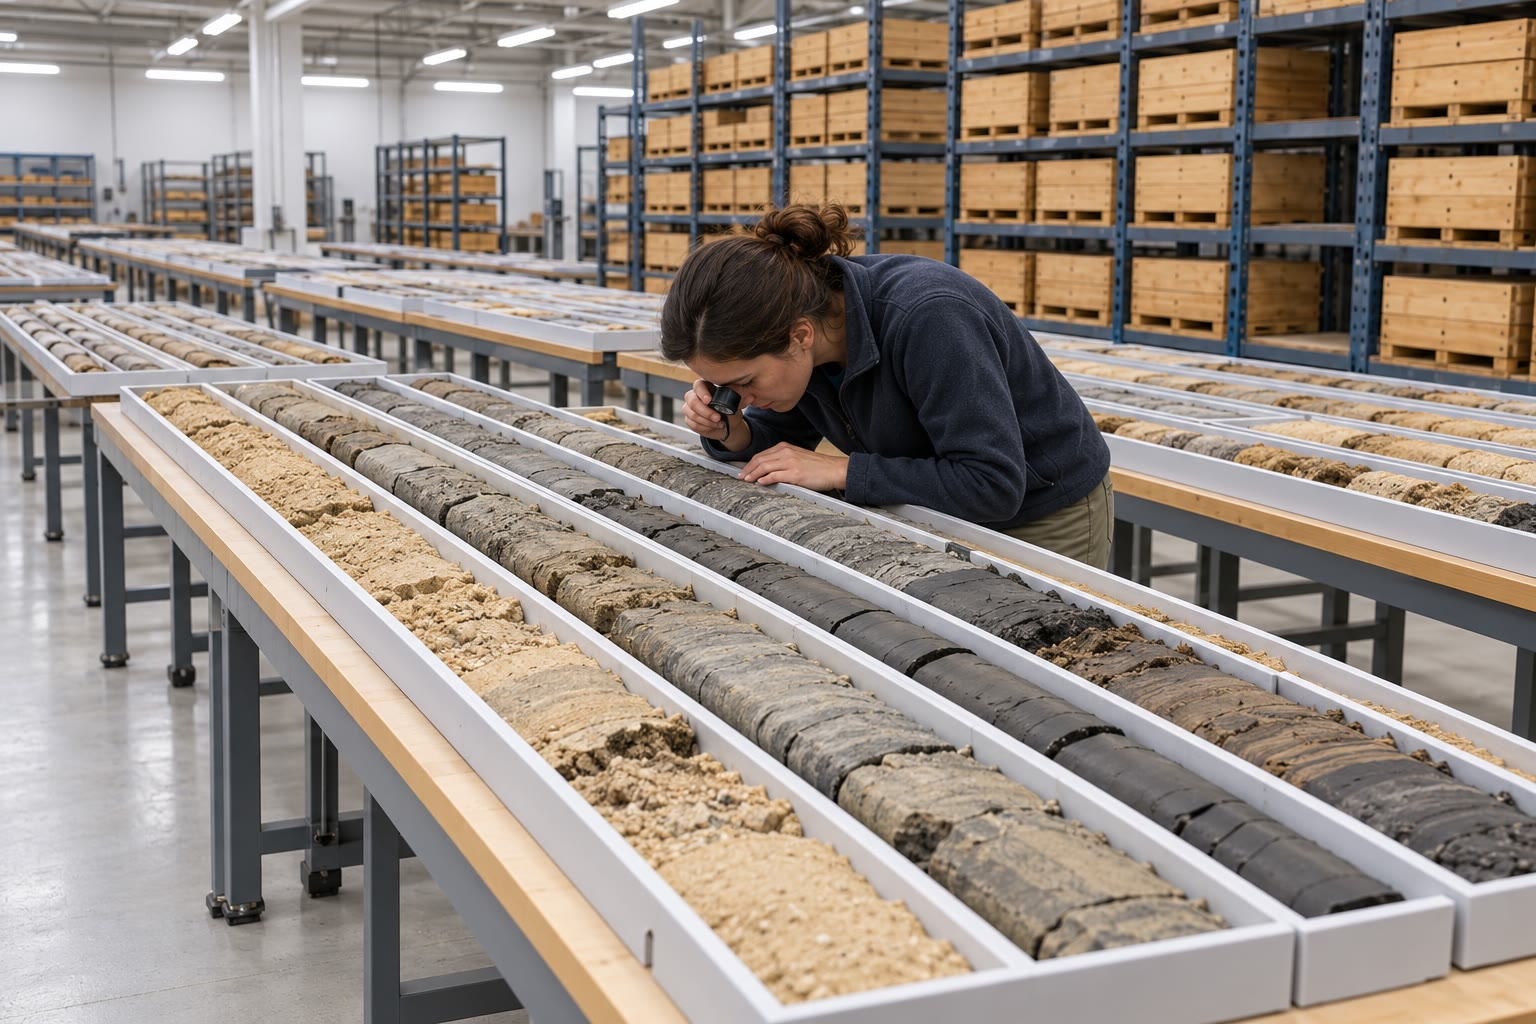
\includegraphics[width=\linewidth]{images/book5/ai/b3-core-store.jpg}

{\scriptsize 岩芯库：托盘中为剖开的砂质与泥质岩芯，一位地质学家
手持放大镜。AI 生成的示意图。}
\end{minipage}
\end{inthelab}

\section{练习}

\begin{exercise}[$\star$]\label{exo:b3:facies-models:1}
某岩芯自下而上显示：离岸泥、泥与细砂互层、
\omterm{def:b3:facies-models:shoreface}{临滨}砂、海滩砂，再上为带根痕的煤层。依据沃尔瑟相律，
给出当时沿海岸的环境排列次序，以及
海岸线移动的方向。若发生海侵，会留下什么沉积？
\end{exercise}

\begin{exercise}[$\star$]\label{exo:b3:facies-models:2}
三个砂体的自然伽马曲线形态分别为：(a) 厚 \qty{8}{m} 的钟形，底界
清晰；(b) 厚 \qty{20}{m} 的漏斗形；(c) 厚 \qty{30}{m} 的圆柱形，
顶底界线清晰。请为每个砂体推断一种沉积环境，并
指出能够证实该推断的岩芯观察结果。
\end{exercise}

\begin{exercise}[$\star$]\label{exo:b3:facies-models:3}
某砂岩的 $\rho_b = \qty{2.40}{g/cm^3}$。以石英为基质、淡水为孔隙流体，求其
孔隙度；再以密度为 \qty{1.1}{g/cm^3} 的卤水代替淡水，重新求解。
\end{exercise}
% ledger: keys:density-porosity

\begin{exercise}[$\star$]\label{exo:b3:facies-models:4}
众数波长分别为 \qty{75}{m} 与 \qty{110}{m} 的波（取自浮标研究中的避风海域与开阔海域），
试估算每种波在何深度处仍保留其表面运动的
\qty{4}{\percent}，以及在深度
\qty{20}{m} 处残留的比例。
\end{exercise}
% ledger: losspeters10:wavebase

\begin{exercise}[$\star\star$]\label{exo:b3:facies-models:5}
某石灰岩的 $\Delta t = \qty{60}{\micro\second/ft}$。求其
孔隙度，采用时间平均方程，基质分别取 47.6 与
\qty{52.6}{\micro\second/ft}，卤水取 \qty{189}{\micro\second/ft}。
这一差异说明了什么？
\end{exercise}
% ledger: keys:sonic

\begin{exercise}[$\star\star$]\label{exo:b3:facies-models:6}
某 \qty{40}{m} 层段中，砂层厚度分别为 6.0、3.5、8.0 与 \qty{2.5}{m}，
均低于截止值，其余为泥。求其\omterm{def:b3:facies-models:ntg}{净毛比}。
若砂层孔隙度为 \qty{22}{\percent}，则该层段每
平方千米所含的孔隙体积为多少？
\end{exercise}

\begin{exercise}[$\star\star$]\label{exo:b3:facies-models:7}
峡谷口附近的一层浊积岩为 \qty{1.2}{m} 厚的块状砂岩，
即 (Ta)，顶部被上覆一层侵蚀；沿扇体向下 \qty{30}{km} 处，同一股浊流形成的一层
厚 \qty{8}{cm} 的波纹层理细砂与粉砂，其上覆
\qty{3}{cm} 厚的泥。指出两层各自的划分，并解释二者的变化。
\end{exercise}

\begin{exercise}[$\star\star$]\label{exo:b3:facies-models:8}
一个厚 \qty{9}{m} 的\omterm{def:b3:facies-models:association}{向上变细序列}，底界清晰，底部含卵石，
向上依次为交错层理砂、波纹细砂与带根痕的泥。解释其成因，并
估算形成该序列的河道深度。沃尔瑟相律能否
应用于其底界？为什么？
\end{exercise}

\begin{exercise}[$\star\star$]\label{exo:b3:facies-models:9}
某台地底面在 \qty{40}{km} 内下降 \qty{60}{m}；另一台地
其水深在 \qty{30}{km} 内保持 \qty{5}{m}，随后在
\qty{1.5}{km} 内下降 \qty{300}{m}。求两者的梯度，命名各台地，并
指出第二个台地边缘处预期的沉积相。
\end{exercise}

\begin{exercise}[$\star\star\star$]\label{exo:b3:facies-models:10}
岸线以速度 $v$ 进积，同时相对海平面以速率
$A$ 上升，其\omterm{def:b3:facies-models:shoreface}{临滨}带宽为 $w$。证明垂向序列中\omterm{def:b3:facies-models:shoreface}{临滨}砂的
厚度为 $h = wA/v$。取 $w = \qty{2}{km}$，
$A = \qty{0.2}{m/ka}$ 与 $v = \qty{20}{m/ka}$ 计算该厚度，并说明当
$A = 0$ 时会发生什么。将结果与
第~\ref{ch:b3:sequence-stratigraphy}~章中关于\omterm{def:b3:sequence-stratigraphy:trajectory}{岸线轨迹}的命题作比较。
\end{exercise}

\begin{exercise}[$\star\star\star$]\label{exo:b3:facies-models:11}
某砂岩的 $\rho_b = \qty{2.30}{g/cm^3}$ 与 $\Delta t =
\qty{86}{\micro\second/ft}$。分别由两种\omterm{def:b3:facies-models:wireline}{测井曲线}求其孔隙度，取石英砂岩
基质（2.65，\qty{52.6}{\micro\second/ft}），孔隙流体为卤水（密度取 1.0，
声波时差为 \qty{189}{\micro\second/ft}）。若声波孔隙度正确，
则\omterm{def:b3:facies-models:wireline}{密度测井}隐含的颗粒密度为多少？胶结物可能是什么？
\end{exercise}
% ledger: keys:density-porosity, keys:sonic

\begin{exercise}[$\star\star\star$]\label{exo:b3:facies-models:12}
在一段岩芯中，黑色离岸泥直接覆于带根的煤层之上，二者接触处
有一薄层贝壳碎屑。解释沃尔瑟相律为何不能跨该界面应用，
说明该界面是何种面，并估算
若海岸线经过时波浪将底面侵蚀至\omterm{def:b3:facies-models:shoreface}{正常浪基面}，则沿岸层序
可能缺失多少，此处\omterm{def:b3:facies-models:shoreface}{正常浪基面}约深 \qty{10}{m}。
\end{exercise}

\section{问题：穿过盖层的 瓦尔登-2 井}

\begin{problem}[{周末问题——一口虚构井的测井曲线、孔隙度、沉积相与净砂，
位于瓦尔登向斜中}]
\label{pb:b3:facies-models:1}
井 瓦尔登-2 钻于瓦尔登丘陵的向斜中，位于
区域网格上的 (7500, 7000) 处，自地面标高
\qty{441.0}{m} 起钻，钻至总深 \qty{1200}{m}。其\omterm{def:b3:facies-models:wireline}{测井曲线}绘于
上一节的图中。颗粒密度分别取 2.65（石英）与
\qty{2.71}{g/cm^3}（方解石），孔隙水密度取 \qty{1.0}{g/cm^3}，基质
声波时差分别为 52.6（砂岩）与 \qty{47.6}{\micro\second/ft}
（石灰岩），水的声波时差取 \qty{189}{\micro\second/ft}。

\medskip\noindent\textbf{第一部分——读取\omterm{def:b3:facies-models:wireline}{测井曲线}。}
\begin{enumerate}
\item 自然伽马值在 \qty{766}{m} 处由 12 跃升至 \qty{110}{API}，
  在 \qty{866}{m} 处降至 18，自 \qty{1046}{m} 起变得不规则，
  自 \qty{1166}{m} 起稳定在 \qty{85}{API}。根据\omterm{def:b3:facies-models:wireline}{测井曲线}，指出所钻遇的各单元。
\item 求盖层各单元的厚度，以及
  盖层底界的标高。
\item 白垩在近地表处读数为 \qty{2.03}{g/cm^3}，
  在 \qty{750}{m} 处为 \qty{2.36}{g/cm^3}。求两个深度处的孔隙度。
  随深度增加，白垩发生了什么变化？
\item 为何不能由页岩的密度求其孔隙度？
\item 片岩读数为 \qty{2.75}{g/cm^3}，声波时差为 \qty{50}{\micro\second/ft}。
  这一声速快、密度高且无孔隙的基底，对钻井人员说明了什么？
\end{enumerate}

\medskip\noindent\textbf{第二部分——孔隙度。}
\begin{enumerate}[resume]
\item 石灰岩读数为 \qty{2.573}{g/cm^3}，求其密度孔隙度。
\item 其声波时差读数为 \qty{58.9}{\micro\second/ft}，求其声波孔隙度，并
  与之比较。
\item 河道充填中的洁净砂读数为 \qty{2.32}{g/cm^3}，求其
  孔隙度。
\item 用其声波时差 \qty{79.9}{\micro\second/ft} 进行核对。
\item 若孔隙水为密度 \qty{1.1}{g/cm^3} 的卤水，则该砂的密度孔隙度
  将改变多少？
\item 哪一个单元更适合作含水层或储层，哪一个
  适合作其上方的盖层？
\end{enumerate}

\medskip\noindent\textbf{第三部分——沉积相。}一段岩芯取自 1108 至
\qty{1124}{m} 深处，自底向上依次为：冲刷面，面上有泥砾和
卵石；\qty{10.4}{m} 厚的交错层理中砂；\qty{3.2}{m} 厚的具波痕细砂，
向上渐变为粉砂；\qty{2.4}{m} 厚的红褐色泥，含根迹。
\begin{enumerate}[resume]
\item 画出取心段内预期的自然伽马曲线形态。
\item 命名各部分的层序及其沉积环境。
\item 运用沃尔瑟定律，描述并排分布的各沉积环境。
\item 估算该河道的深度。
\item 该砂岩含十一个此类单元，每个单元的底界均为突变界面。
  其叠加方式说明了该河流及其平原的哪些情况？
\item 能否用沃尔瑟定律由一个单元推至下一个单元？为什么？
\end{enumerate}

\medskip\noindent\textbf{第四部分——净砂。}十一个河道充填体，
自砂岩底部起，厚度依次为 14、9、12、7、16、10、13、8、11、12 和
\qty{8}{m}。每个充填体下部为清洁砂（\qty{30}{API}），占其厚度的
0.60、0.45、0.55、0.30、0.65、0.40、0.55、0.35、0.50、
0.45 和 0.30；其上为向上变细段，占其厚度的 0.25、0.30、0.25、0.40、
0.20、0.30、0.25、0.35、0.25、0.30 和 0.35，自然伽马值线性升至
\qty{105}{API}，顶部以泥岩结束。
\begin{enumerate}[resume]
\item 各向上变细段中，哪一部分位于 \qty{60}{API}
  截止值以下？
\item 计算最底层单元与最厚单元的净砂厚度。
\item 计算该砂岩中清洁砂总厚度与
  向上变细段总厚度。
\item 计算其\omterm{def:b3:facies-models:ntg}{净毛比}。
\item 若截止值分别取 45 或
  \qty{75}{API}，净砂厚度将如何变化？
\item 取问题 8 中砂的孔隙度，计算
  每平方千米范围内净砂的孔隙体积。
\item 写出 瓦尔登-2 井处三叠纪砂岩的净砂厚度。
\end{enumerate}
\end{problem}
% ledger: keys:density-porosity, keys:sonic, keys:gamma
